%!TEX root = report.tex
\chapter{Other Technical Details}


\section{Daemen Script Management - Supervisor}

\section{Scheduled Tasks Management - Jenkins}
\par We used Jenkins\cite{jenkins} to managed our predictions timetable update schedule.
\todo[inline]{add screenshots for jenkins}


\subsection{Current Timetable Update}
\par The current timetable is re-generated every hour. We set up a Jenkins job to re-run the relevant current timetable update SQL script every hour, and save the previous timetable into a log for updating the historical timetable at a later time. This job takes less than 10 minutes on average.

\subsection{Historical Timetable Update}
\par Similarly, we set up a Jenkins job to update the Historical Timetable daily at 3.30am when the server is less busy.

\subsection{Arrivals Daily Backup}
\par The arrivals table grows rapidly by approximately 150 thousand rows per hour. In order to allow fast access to the arrivals within the past one hour to construct the current timetable, we decided to save the arrivals for the current day in a new table, while keeping the past arrivals entries in an archive table. This required us to backup the arrivals entries daily to the arive.

\par Again, we created a Jenkins job to run the back up script daily. In order not to affect the historical timetable update, we set this job as a downstream task of the historical timetable update.

\subsection{Software Project Management - Trello}
\par We used Trello \cite{trello} for project management. It was useful to keep track of the tasks backlog, the tasks at hand, and the tasks to be further tested (Figure \ref{fig:trello}).

\begin{figure}
\centering
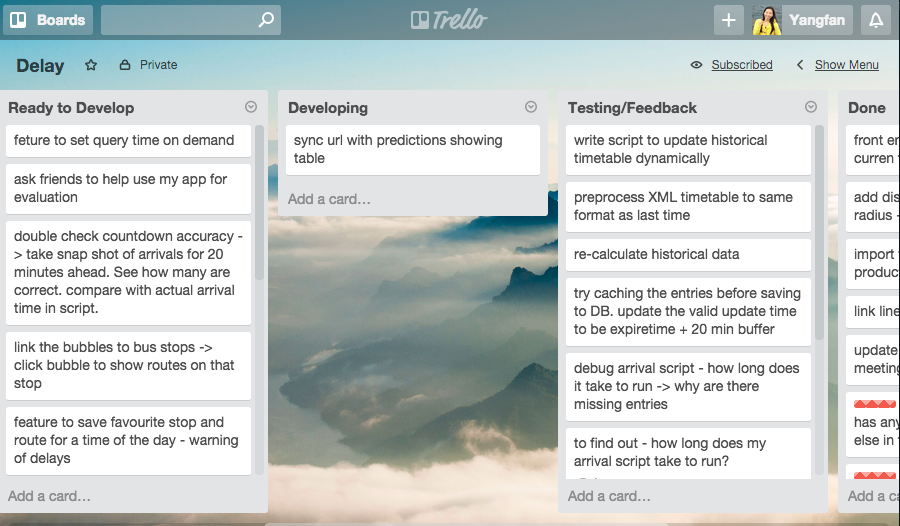
\includegraphics[width=\textwidth]{figures/trello_small.png}
\caption{\label{fig:trello} Project Trello Board}
\end{figure}
